\documentclass[margin=5mm]{standalone}
\usepackage[dvipsnames]{xcolor}
\usepackage{pgfplots}
\usepackage{tikz}
\usepackage[tikz]{ocgx2}

\pgfplotsset{compat=1.18}
\begin{document}

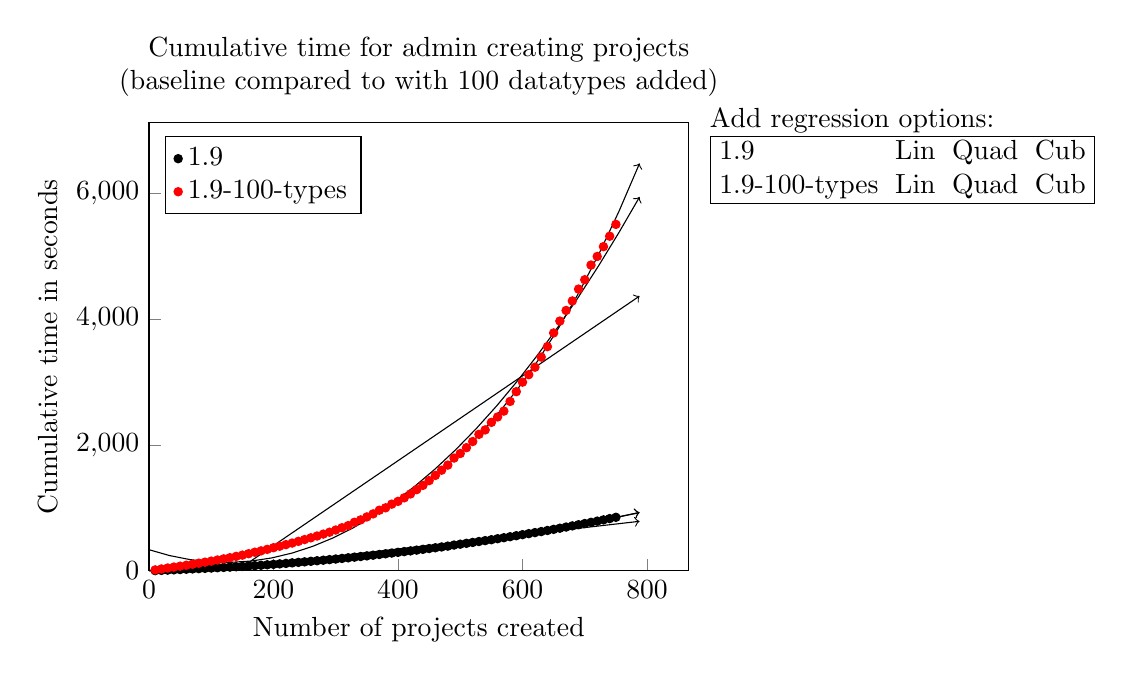
\begin{tikzpicture}
    \begin{axis}[
        align = center,
        legend pos = north west,
        legend cell align = left,
        xlabel = Number of projects created,
        ylabel = Cumulative time in seconds,
        xtick pos = left,
        ytick pos = left,
        scaled ticks = false,
        xmin = 0,
        ymin = 0,
        title = {Cumulative time for admin creating projects (baseline compared to with 100 datatypes added)},
        title style = {text width = 0.8\textwidth},
        legend entries={\switchocg{1.9}{1.9},\switchocg{1.9-100-types}{1.9-100-types}}]
        \begin{scope}[ocg = {ref = 1.9-Lin, status = invisible}]
            \plot[domain=0:788,->,forget plot] (\x,{-105.2838212612613091323510161601006984710693359375 + 1.1335993541963016451035173304262571036815643310546875*(\x)^1});
        \end{scope}
        \begin{scope}[ocg = {ref = 1.9-Quad, status = invisible}]
            \plot[domain=0:788,->,forget plot] (\x,{6.74133892632342135442513608722947537899017333984375 + 0.260676028059277531401249916598317213356494903564453125*(\x)^1 + 0.00114858332386450563873669938885768715408630669116973876953125*(\x)^2});
        \end{scope}
        \begin{scope}[ocg = {ref = 1.9-Cub, status = invisible}]
            \plot[domain=0:788,->,forget plot] (\x,{4.04437001110679883453258298686705529689788818359375 + 0.301900793458898697441128433638368733227252960205078125*(\x)^1 + 0.00101386959183570276622765593543817885802127420902252197265625*(\x)^2 + 0.00000011816994037614292616206689533198126440538544557057321071624755859375*(\x)^3});
        \end{scope}
        \begin{scope}[ocg = {ref = 1.9, status = visible}]
            \addplot[
                only marks,
                color = black,
                mark = *,
                mark size = 1.5 pt
            ]coordinates {(10,4.931)(20,9.134)(30,13.311)(40,17.695)(50,22.294)(60,27.594)(70,31.937)(80,36.691)(90,41.222)(100,45.845)(110,50.812)(120,55.68)(130,60.726)(140,66.37)(150,71.829)(160,77.868)(170,83.797)(180,90.383)(190,97.513)(200,105.053)(210,112.256)(220,119.659)(230,128.257)(240,136.179)(250,144.341)(260,153.19)(270,161.802)(280,170.596)(290,179.841)(300,188.936)(310,198.617)(320,208.469)(330,218.894)(340,228.812)(350,239.291)(360,250.011)(370,261.132)(380,272.497)(390,284.112)(400,295.353)(410,306.839)(420,318.225)(430,330.469)(440,342.996)(450,355.568)(460,368.001)(470,380.75)(480,394.065)(490,411.124)(500,424.877)(510,438.667)(520,452.582)(530,467.231)(540,481.342)(550,495.692)(560,511.606)(570,527.461)(580,543.285)(590,559.377)(600,575.898)(610,592.178)(620,608.772)(630,625.275)(640,642.524)(650,660.281)(660,678.336)(670,697.09)(680,715.445)(690,733.601)(700,752.733)(710,771.703)(720,790.871)(730,810.921)(740,830.933)(750,851.647)};
        \end{scope}
        \begin{scope}[ocg = {ref = 1.9-100-types-Lin, status = invisible}]
            \plot[domain=0:788,->,forget plot] (\x,{-945.2441412612606654874980449676513671875 + 6.73837577524893216462942291400395333766937255859375*(\x)^1});
        \end{scope}
        \begin{scope}[ocg = {ref = 1.9-100-types-Quad, status = invisible}]
            \plot[domain=0:788,->,forget plot] (\x,{337.46858234727784520146087743341922760009765625 + -3.256788304817607393459866216289810836315155029296875*(\x)^1 + 0.01315153168429808276662651422839189763180911540985107421875*(\x)^2});
        \end{scope}
        \begin{scope}[ocg = {ref = 1.9-100-types-Cub, status = invisible}]
            \plot[domain=0:788,->,forget plot] (\x,{-25.955972155167639670025891973637044429779052734375 + 2.2983710132206507381624760455451905727386474609375*(\x)^1 + -0.0050015429661738053379593793579260818660259246826171875*(\x)^2 + 0.00001592374969339639898262446504606515418345225043594837188720703125*(\x)^3});
        \end{scope}
        \begin{scope}[ocg = {ref = 1.9-100-types, status = visible}]
            \addplot[
                only marks,
                color = red,
                mark = *,
                mark size = 1.5 pt
            ]coordinates {(10,16.405)(20,31.46)(30,46.593)(40,61.432)(50,75.75)(60,90.651)(70,106.319)(80,123.32)(90,139.44)(100,156.124)(110,173.693)(120,191.673)(130,210.425)(140,230.973)(150,250.881)(160,273.495)(170,297.303)(180,318.672)(190,342.808)(200,368.579)(210,392.646)(220,417.758)(230,442.898)(240,469.85)(250,498.114)(260,525.813)(270,554.65)(280,584.927)(290,614.842)(300,649.698)(310,686.267)(320,719.936)(330,772.646)(340,810.658)(350,857.787)(360,905.979)(370,963.999)(380,1002.261)(390,1060.688)(400,1104.422)(410,1161.154)(420,1222.425)(430,1290.711)(440,1358.457)(450,1434.036)(460,1517.043)(470,1599.521)(480,1680.728)(490,1791.95)(500,1864.981)(510,1956.855)(520,2054.818)(530,2168.158)(540,2238.968)(550,2359.04)(560,2444.432)(570,2537.774)(580,2691.543)(590,2846.338)(600,2997.482)(610,3115.962)(620,3235.05)(630,3395.595)(640,3561.225)(650,3778.986)(660,3967.71)(670,4135.584)(680,4287.09)(690,4475.074)(700,4623.899)(710,4856.898)(720,4993.503)(730,5148.716)(740,5314.463)(750,5502.395)};
        \end{scope}
    \end{axis}
    \begin{scope}
        \addtolength{\tabcolsep}{-0.3em}
        \node [below right, shape=rectangle, align=left](regressiontable) at (7,6) {
            Add regression options: \\
            \begin{tabular}{|llll|}
                \hline
                1.9 & \switchocg{1.9-Lin}{Lin} & \switchocg{1.9-Quad}{Quad} & \switchocg{1.9-Cub}{Cub} \\
                1.9-100-types & \switchocg{1.9-100-types-Lin}{Lin} & \switchocg{1.9-100-types-Quad}{Quad} & \switchocg{1.9-100-types-Cub}{Cub} \\
                \hline
            \end{tabular}
        };
    \end{scope}
\end{tikzpicture}

\end{document}